\documentclass{standalone}
\usepackage[dvipsnames,svgnames,x11names]{xcolor}
\usepackage{tikz}
\usepackage{pgfplots}
\pgfplotsset{compat = 1.12}
\usepackage{../thesismath}
\begin{document}
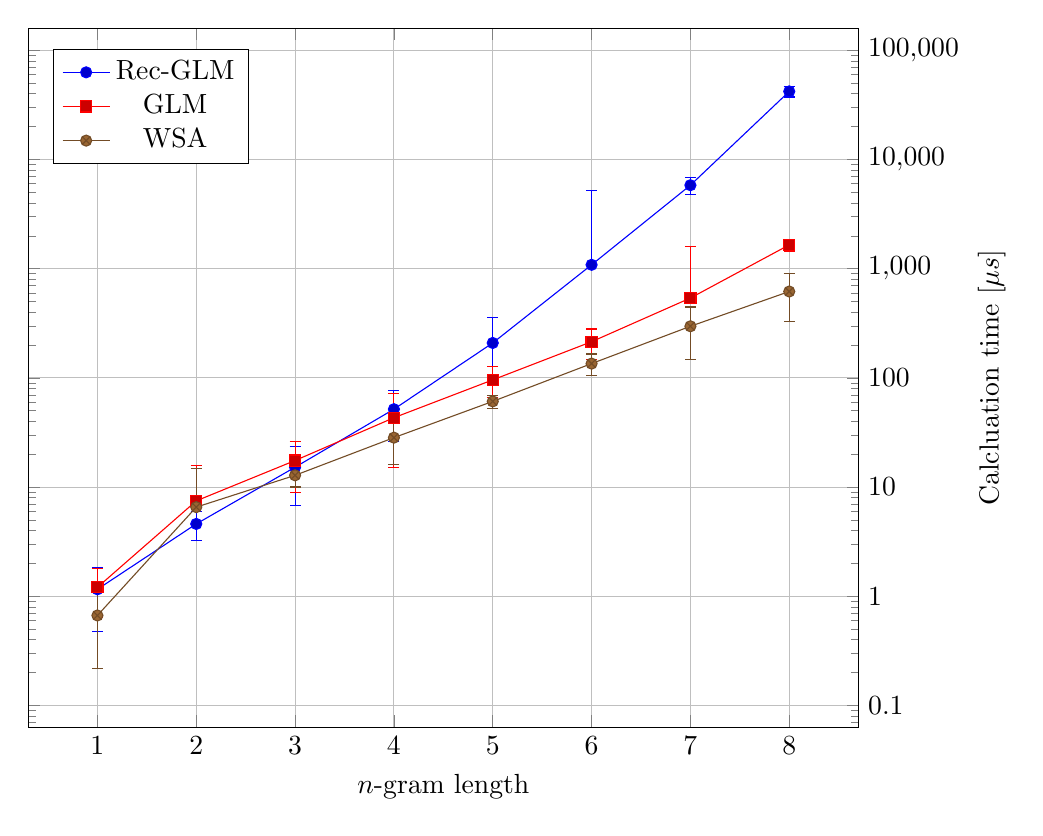
\begin{tikzpicture}[baseline]

\begin{axis}[
  xlabel = {$n$-gram length},
  xtick = {1, ..., 8},
  ylabel = {Calcluation time [$\mu s$]},
  yticklabel pos = right,
  ymode = log,
  log ticks with fixed point,
  %yticklabel pos = right,
  minor y tick num = 4,
  grid = major,
  legend entries = {{Rec-GLM}, {GLM}, {WSA}},
  legend pos = north west,
  width = \textwidth,
]

% Rec-GLM
\addplot+[
  error bars/.cd,
  y dir = both,
  y explicit,
] table [y error = us_error] {
  n  us         us_error
  1      1.158     0.678
  2      4.596     1.372
  3     15.200     8.459
  4     51.656    25.336
  5    208.875   148.245
  6   1085.126  4135.734
  7   5814.210  1020.824
  8  42025.650  4621.103
};

% GLM
\addplot+[
  error bars/.cd,
  y dir = both,
  y explicit,
] table [y error = us_error] {
  n  us         us_error
  1      1.207     0.574
  2      7.475     8.341
  3     17.503     8.631
  4     43.166    28.144
  5     95.882    30.063
  6    214.342    65.797
  7    538.550  1064.181
  8   1652.884   210.847
};

% WSA
\addplot+[
  error bars/.cd,
  y dir = both,
  y explicit,
] table [y error = us_error] {
  n  us         us_error
  1      0.667    0.451
  2      6.548    8.214
  3     12.810    2.805
  4     28.359   12.223
  5     60.901    8.288
  6    135.130   30.505
  7    296.816  149.366
  8    618.084  289.517
};

\end{axis}

\end{tikzpicture}
\end{document}
